\documentclass[a4paper]{llncs}
\usepackage{printlen} % Print lengths using specified units. 
%\usepackage{hyperref}
\usepackage{booktabs}
\usepackage[utf8]{inputenc} % Umlaute üöä auch normal benutzen und nicht maskieren
\usepackage{color}
% http://www.ctan.org/tex-archive/fonts/ps-type1/cm-super/
\usepackage[T1]{fontenc} % use high quality fonts, please install cm-super
\usepackage[pdftex]{graphicx}
\graphicspath{{./Depictions/}}
\DeclareGraphicsExtensions{.pdf,.jpeg,.jpg,.png}
\usepackage[T1]{url}
\usepackage{listings}
\usepackage{subfig}
\usepackage{printlen} % Print lengths using specified units.
\usepackage{booktabs}
%\usepackage[textsize=tiny]{todonotes}
\usepackage{todonotes}

\usepackage[
pdftex,
bookmarks=true,
%hidelinks,
unicode=true,
pdfauthor={Sebastian Tramp, Henry Story, Andrei Sambra, Philipp Frischmut, Michael Martin, and S\"oren Auer},
pdftitle={Extending the WebID Protocol with Access Delegation},
pdfkeywords={WebID, Social Semantic Web, Access Delegation}
]{hyperref}

\title{Extending the WebID Protocol with Access Delegation}

\author{Sebastian Tramp\inst{1} \and Henry Story\inst{2} \and Andrei Sambra\inst{3} \and Philipp Frischmuth\inst{1} \and Michael Martin\inst{1} \and S\"oren Auer\inst{1}}

\institute{
Universit\"at Leipzig, Institut f\"ur Informatik, AKSW,\\
Postfach 100920, D-04009 Leipzig, Germany,\\
\email{\{lastname\}@informatik.uni-leipzig.de}\\
\url{http://aksw.org/FirstnameLastname} (WebID)
\medskip\and
Apache Foundation\\ 
\email{henry.story@bblfish.net}\\
\url{http://bblfish.net/people/henry/card\#me} (WebID)
\medskip\and
CNRS Samovar UMR 5157, TELECOM SudParis\\
\email{andrei.sambra@it-sudparis.eu}\\
\url{https://my-profile.eu/people/deiu/card\#me} (WebID)
}

\authorrunning{Sebastian Tramp et al.}

%%%%% LISTINGS
\usepackage{listings} % Typeset source code listings using LaTeX.
% listing styles
\lstset{%
    numberbychapter=false,
    numberblanklines=true,
    numbers=left,
    numberstyle=\tiny,
    basicstyle=\ttfamily\footnotesize,
    emphstyle=\textit,
    tabsize=2,
    framexleftmargin=2pt,
    captionpos=b,
    frame=single,
    breaklines=true
}
\lstdefinestyle{rdf}{morekeywords={}}
\lstdefinestyle{sparql}{
    morekeywords={SELECT,OPTIONAL,FROM,DISTINCT,a,WHERE,FILTER,GROUP,ORDER,LIMIT,BY,IN,AS},
    emph={s,p,o}
}
\lstdefinestyle{turtle}{
    morekeywords={a, @prefix, cert,xsd,foaf, rdf, rdfs, owl},
    morecomment=[s][\textrm]{<}{>},
    morecomment=[s][\textit]{"}{"},
}

\begin{document}

\maketitle              % typeset the title of the contribution

\begin{abstract}
The WebID protocol enables the global identification of agents in a distributed manner by combining asymmetric cryptography and Linked Data.
WebIDs are mostly used in scenarios where a user utilize a browser application to access a protected resource on a web server.
But in order to decide whether access should be granted or denied, the web server itself needs to retrieve other WebID profiles and linked resources in order to work out if the requesting agent is part of the authorization group ( eg: is a friends of a friend of the resource owner ).
It would seem that at present this information needs to be publicly available for the server to access it. This  leads to a privacy issue, since agents may want to limit access to a users social graph.
In this paper we propose an extension to the WebID protocol which allows for delegation of access authorization from a WebID to a third party, e.g. allowing a server to be able to act on behalf of its users.
This extends the range of application scenarios where WebID authentication can be efficiently deployed while increasing privacy.
\end{abstract}

% this prints the current textwidth, so images can be
% generated perfectly fitting to the page (LNCS textwidth: 121.99854 mm)
%\uselengthunit{mm}\printlength{\textwidth}
%\uselengthunit{mm}\printlength{\columnwidth}

\section{Introduction}\label{sec:intro}

The World Wide Web is a peer to peer communication system designed from the outset to work in a global space, between agents distributed around the world and acting in parallel, with no center of control, in a space where new agents can at any point join and there is no complete overview of the whole system.
These agents need know nothing of each other up to the point of their interaction.
This is the force that leads the web to its declarative functional architecture, with its emphasis on naming and a logic of unalterability of the meaning of names (URIs).  
  
Agents on the web communicate with each other through a limited number of actions: by making requests for resources (GET), by creating resources (POST or PUT), or even by deleting resources \ldots
Creation or deletion of resources usually require authentication of the agent making the request, and so in many cases do requests for information (GET). 

The WebID protocol enables the global identification of agents using asymmetric cryptography in a way that fits cleanly with this architecture: namely in such a way that agents can verify each others identity without having had any previous interactions and in such a way as to allow trust to build up in a decentralized manner.

A \textit{WebID} is a URI that refers to an agent - person, robot, group or other thing that can have intentions.
The WebID should be a URI which when dereferenced returns a representation whose description uniquely identifies the agent as the controller of a public key~\cite{sporny-m-2011--a,story-h-2009--a}

The WebID protocol is used currently mostly for client authentication%
\footnote{Server authentication using IETF DANE follows much the same logic, except that the lookup for the identity is not done using the HTTP protocol but DNSSEC.}.
It is worth noting that the host serving the WebID profiles controls the identity of every agent whose URI is within that server's namespace.
This service is known as the origin server~\cite{barth-a-2011--a}.
It is the origin of all resources served by it. 

We can easily think of the origin server as not only able to respond to requests, but also as an agent able to make requests.
Indeed WebID authentication requires the server to make WebID profile requests to other servers in order to verify the identity of agents making a request to it.
The WebID spec describes this task as being accomplished by a separate agent, the WebID verifier - which could indeed be done by another service on the web (WebID proxy authentication servers).
But it can also be so closely tied to the web service that it would be natural to think of it as part of that same service.
The WebID profile furthermore could be served by the same agent as the one making the request, in which case we have a minimal case of a peer to peer communication.
Note that fetching a WebID profile for WebID authentication should be done anonymously, for fear of authentication deadlocks.\footnote{ for example one can imagine an agent S  with profile Ps requesting a resource on server R which requires authentication. S would send R its certificate, thereby requiring  R to dereference S's Profile Ps in order to verify the WebID. If Ps  itself requires authentiction of R and if R sends a certificate containing a WebID with its profile Pr, and if Pr itself requires authentication then it looks like we have a deadlock.  }

Things get more interesting in the authorization space.
Consider a very natural application of WebID: allowing friends of one's friends (foaf) access to some resources.
This authorization rule will require the web server to fetch each of its users' friends profiles, in order to build up such a list.
But there is a privacy issue involved here: not every one wants to make all of their social network publically visible, and some may not want to make any of it publicly visible.
Those people may then protect their FOAF profile with access control rules.
How can a server that needs access to these FOAF profiles in order to apply its own access control rules - such as only allowing access to foaf - get access to the information?
Should it be able to do so?
These are the questions we will try to answer in this paper.

The rest of the paper is organized in the following way:
\autoref{sec:req} describes the usage scenario and additional requirements which we had in mind for our solution,
\autoref{sec:spec} goes into detail with the WebID specification and adds support for authorization delegation,
in \autoref{sec:eval} we describe our reference implementations based on two web applications and finally
in \autoref{sec:relatedwork} we compare our proposal with two protocols, namely CORS and OAuth.


%\section{Terminology}
%\textit{Access Delegation} is a relation between two WebID resources.
%The relation describes, under which circumstances a secretary agent has access to a certain resource under the same constraints as the named agent.
%The secretary agent declares to act in the name of the named agent.

\section{Requirements}\label{sec:req}

This section describes several usage scenarios requiring access delegation which can not be solved efficiently with the standard WebID authentication protocol.
In addition to that, we list derived implementation requirements.

%\subsection{Basic Use-Cases for Access Delegation} \label{sec:usecases}

%\subsubsection{Personal Devices and Applications}

Currently, the default usage intention for WebIDs consists of browser-based authentication scenarios.
This is an important use-case and should be of special interest since we use the World Wide Web not only through browsers but also through other applications as well as other application on other devices such as smartphones, tablets and freedomboxes\footnote{\url{https://freedomboxfoundation.org/}}.
In a typical every day usage scenario, we use feed readers and social network clients hand in hand with web browsers.
All these applications act in the name of their users and fetch and manipulate resources in a way as if it were done by the users themselves and with her browser.
These applications provide their services to one user only and also run on a device which is commonly accessed by one user only (e.g. a smartphone).
This class of \textit{private applications} is similar to browsers and can be seen as an extension to the user itself~\cite{clark-a-1998-7-a}.

As a slightly different case, we can identify the class of \textit{service applications}.
These applications also manipulate resources in the name of the user but they do this for more than one user.
These services are hosted by a third party e.g. not by the user itself, nor by the owner of the protected resource where our user has an interest in.
In addition to that, we argue that the level of trust which is given by a user is lower than to an application which runs on a personal device and can be turned off by herself.
A typical application domain for this class of applications is the Social Web, and more specifically, the distributed and semantic Social Web.
In this infrastructure, multiple services such as photo sharing, recipe management or todo lists create and manipulate artefacts like notes, comments and images and spin a data network based on a Linked Data infrastructure and shared vocabularies~\cite{tramp-s-2012--a}.

In this paper will show that this class of service applications can not handle access delegation efficiently without an extension to the protocol such as the one we propose.

%\subsubsection{Vacation Replacement}

%I a typical office scenario, employees declare vacation replacements for the time of their holiday in order to achieve an uninterrupted service during that time.

%One option to allow access to the vacation replacement user is to give him the original certificate or to add his private key to the users WebID.
%This solution has two drawbacks: (1) the users certificate is burned after the vacation and she needs to create a new one, (2) a resource guard can not distinguish between the user and the vacation replacement user, which allows for abuse.
%In this context, the named agent is the employee which is on holiday and her vacation replacement is the secretary agent.

%\subsubsection{Groups and Roles}

%Access for \textit{working groups} to a resource is typically specified in a way that each resource guard needs to maintain an owned or cached list of group members of this group.
%In the Social Semantic Web, these working groups have its own WebID resources which describe the group as an entity and its members as relations to their user WebIDs.
%To authorize a group of agents to access a resource should be as simple as to authorize a single agent.

%In order to allow this, we define the group as the named agent and all group members as its secretary agents.
%An alternative could be to share one single group certificate with all members or to create a group certificate for each member and describe all public keys in the group WebID.
%Again, these solutions have different drawbacks: (1) a shared certificate needs to be updated each time a user leaves the group, (2) multiple group certificates for each user does not allow for distinguishing which user accessed the resource, which allows for abuse. 
%In this context, the group is the named agent and all current group members are secretary agents.\todo{A: not sure I agree (see source)}%the group is not an entity, therefore it cannot take actions by iteself. Actions are always performed by users, as part of the group.

%An \textit{office role} is a slightly different construct where a user can access specific resources because of his working description.
%A product manager has access to all product related resources because of her role as product manager and not because of her identity.
%The role itself is identified by a WebID and all access authorization rules should use this WebID instead of a user WebID.

%In this context, the role is the named agent and the current role owner is the secretary agent.

%\subsection{Implementation Requirements}

Based on this usage scenario and additional preliminary considerations, we issue the following implementation relevant requirements for an access delegation solution based on the WebID authentication protocol.
We have identified the following roles being part of the access delegation process:
\begin{enumerate}
    \item The \textit{secretary agent} is the agent which acts in the name of another agent.
This agent actually requests some resources and tries to do that on behalf of someone.
    \item The \textit{named agent} is the agent which is represented by the secretary.
This agent does not have an active role in the request but is named as the origin of the activity.
\end{enumerate}
In the following requirements list, we use both terms consequently to avoid confusion.

\subsubsection{Distinguish secretary agents from named agents}
Delegation should not be handled by camouflaging an request of an agent in the sense that this request is indistinguishable from a named agent request.
A secretary agent should use its own certificate and it should be identified and described by its own WebID profile.
The motivation for this is twofold.
Firstly, it allows resource guards to permit or deny requests based on this information.
Secondly, applications which are secretary for many different named agents do not need to switch their certificate between requests.
Also they do not need to handle hundreds of different keys.

\subsubsection{Easy to use}
The one and only place to describe which secretary agents are allowed to operate as a named agent should be the WebID profile itself.
To grant delegated access to a secretary agent, no other actions than simply adding triples to the WebID profile should be needed.
To reset this grant the same triple can removed from the WebID profile. 

\subsubsection{Linked Data and Read Write Web integration}

The solution we try to architect aims to enhance the communication for consumption and modification of Linked Data esp. from the applications point of view.
This means, that existing Linked Data as well as Read-Write-Web principles should not be violated by the architecture.
\todo{what does rww means here?}

\subsubsection{Minimal protocol footprint}

In addition to the integration requirement, we argue that a minimal protocol footprint should be achieved to allow a wide adoption of the extension.
This includes the requirement to not add an additional service to the process of authentication than using the existing ones.

\todo{ST: add efficency requirement}
%\subsubsection{No enforcement to reveal agent identities}\todo{maybe we kick this ...}
 
%Since we know that social networks play an important role in a context where communication is restricted by different parties, an 

\section{Extending WebID for Access Delegation}\label{sec:spec}

\subsection{Solution 1: Passing itself for the user}

The simplest solution for any agent $S$ wishing to pass itself off as one of the users $U$, is for it to create a public / private key pair,  place the public key in a certificate $C_u$ and add the public key to the users' profile $P_u$.
Having done this the agent $S$ can then connect using the certificate $C_u$ to any service it wishes to, when it wants to work for the user $U$.
This has the advantage of requiring no change to the WebID protocol.
It does give the agent $S$ all powers of the user $U$ and so has to be handled with great care.

What kind of agents does it make sense to give such rights to?
Or put another way: what agent would giving such rights to not constitute a reduction in security to the user?
Or put yet another way: which agent could take such a role at its behest at any moment in any case?
Or: which agent does the user and the authorization server already rely on for authentication?
There is one agent  on which any service requiring WebID authentication relies on and this is the WebID profile origin server~\cite{barth-a-2011--a}.
Any server requiring authentication of an agent using WebID must trust the origin server serving the WebID Profile.
That origin server can at any time change the public keys in the profiles sent back to any authorization agents and indeed change any information in the profile it wants to.
Any user profile can then be thought of as being a user according to the origin server ie a \url{user@origin.org:port} - where \url{origin.org} is the domain of the origin server, and \url{port} is the port the server is running on.

When the user owns the origin server then the origin server is just an extension of the user, and in that case there need be no thought of a difference between the user and the origin server.
In that case the origin server can in fact just authenticate as the user whenever needed.

But when the origin server (OS) is serving a number of different profiles and is acting on behalf of a number of different users, then we have an efficiency issue that rears its head.
Whenever the Origin Server needs to act on behalf of one ifs users to a remote server $R$ it will need to open a new TLS connection to that server using one of its users public keys.
For $N$ users this could require $N$ parallel connections to a server $S$.
\todo{calculate how inefficient this is, and at what size of network this starts really become problematic}
\todo{ST: add disadvantages according to the requirements (identity)}
 
\subsection{Solution 2: Origin Server acting on Behalf of a User}

In order to reduce the number of open connections to any server down to a minimum, it would be useful if the origin server could identify itself directly when making a request and specify on behalf of which of its users it was acting on.
One way would be for the origin server acting as client to simply use the same public key as the origin server acting as server - that is it could use the same public key as the one used by the TLS server.
It could even use the same certificate.
This would make clear to any server it was connecting to, that it could rely on this server as much as it could on the identity of any user served by that server.

Still, such a server connecting to a remote service on behalf of one of its users would then need to identify which user it was acting on behalf of, or the remote service receiving a request would not know which access control rule to apply to the origin server.

After all the remote service may have resources which should be readable by the origin server users $OS_{u1}$ and $OS_{u2}$, but not to the origin server users $OS_{u3}$ and $OS_{u4}$.
Or the representations returned may differ somewhat for each group of users.
$OS_{u1}$ and $OS_{u2}$ may get some more information than $OS_{u1}$ and $OS_{u2}$.
As a result it is important for the origin server to distinguish on behalf of which users it is acting when making a request.

Problems: using the same key between server acting as client and as server risks making the keys available to a wider audience, and so increases the risk of key compromise. 

\todo{insert description of On-behalf-Of header (at least the importance of such a feature)}

\subsection{Solution 3: Secretary acting on Behalf of a User}

The origin server acting as a client on behalf of a user can then be thought of as a keep of secrets for that user.
It should know how to distinguish what remote servers tell it when it is acting on behalf of one user, from what a remote server tells it when it is acting on behalf of another user.
The role of the keeper of secrets for a person is known as the secretary role - a prestigious role taken on for example by figures such as the Secretary of State, Hillary Clinton.

If we now identify the secretary that can act on behalf of a user we can generalise the protocol somewhat.
When the server authenticates as a secretary to a remote server it can use its own WebID.
But how would the remote server know that it can trust that secretary to be acting on behalf of a particular user?
It can no longer just compare the TLS keys.
Instead it can see if the user that the secretary is acting on behalf of has stated clearly that that agent is its secretary.
This can be discovered by checking out the profile... \todo{fill out the details here}

\autoref{fig:AuthSequence} depicts the process of a WebID authentication which is extended with the following components to allow access delegation:

\begin{itemize}
    \item The requesting agent (the secretary) claims a request as requested in the name of a named agent (see point 2).
        This adds a HTTP request header to the specification.
    \item The WebID verifier needs to verify not only one but two different WebID incl. the relation between these two resources (see point 4).
        This adds additional verification rules to the specification.
    \item The named agent (Bob) can declare any relation to his secretary agents in his WebID profile.
        This adds a vocabulary for describing access delegation to the specification.
\end{itemize}

\begin{figure*}[htb]
  \centering
  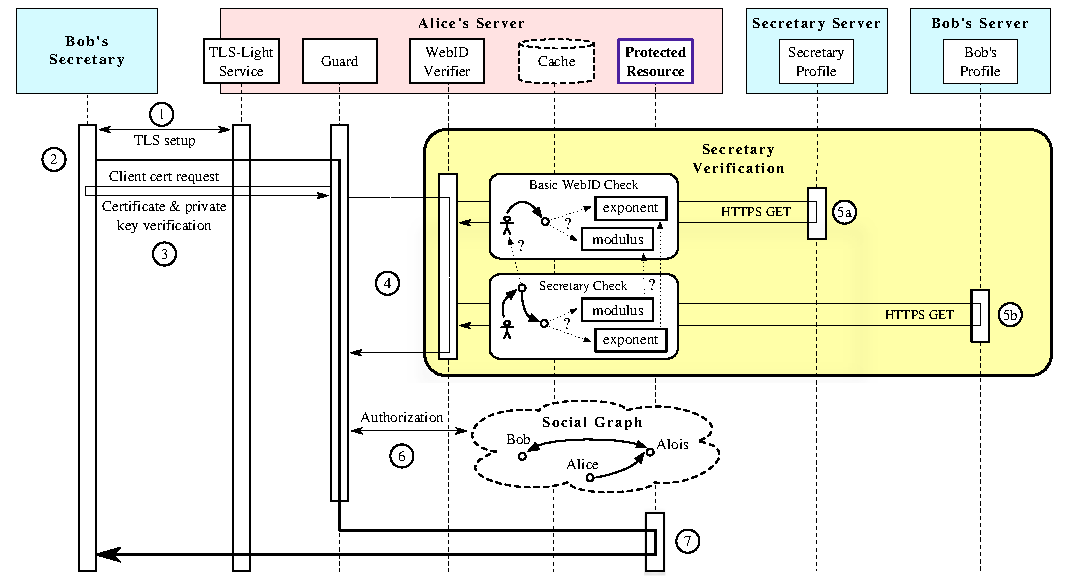
\includegraphics[width=\textwidth]{AuthSequence}
  \caption{Extended WebID authentication sequence}
  \label{fig:AuthSequence}
\end{figure*}

The following enumeration describe each authentication step in detail but concentrates on the context of access delegation:

\begin{enumerate}
    \item Bob's secretary agent opens a TLS connection with the server of the protected resource.
    \item Once TLS is set up, the HTTP request is sent to the server (e.g. a \verb!HTTP GET!) to consume or manipulate a resource.
        Here our first addition comes into play, the HTTP request header to claim an request as a secretary.
        We assume that the guard intercepts this HTTP request, and requests for a client authentication (using the TLS service)
    \item This authentication request is done using public key cryptography, sign a token with the guards private key and have the secretary send its certificate.
        This is defined in the TLS protocol which is specified in \cite{dierks-t-2012--a} and its successive RFCs.
        At the end of this step, the secretaries certificate is handled back to the guard.
    \item The guard ask the verification agent to verify the WebID is named in the certificate.

        %The WebID Certificate is then passed on to the Guard with the proviso that the WebIDs still needs to be verified.
    %The Guard then must ask the Verification Agent to verify that the WebIDs do identify the agent who knows the given public key.
    %The WebID is verified by looking up the definition of the URL at its canonical location. This can be done by dereferencing it. The Verification Agent must extract the public key and all the URI entries contained in the Subject Alternative Name extension of the WebID Certificate. A WebID Certificate may contain multiple URI entries which are considered claimed WebIDs at this point, since they have not been verified. The Verification Agent may verify as many or as few WebIDs it has time for. It may do it in parallel and asynchronously. However that is done, a claimed WebIDs can only be considered verified if the following steps have been accomplished successfully:
        %If the WebID Verifier does not have an up to date version of the WebID profile in the cache, then it must dereference the WebID using the canonical method for dereferencing a URL of that scheme. For an https://... WebID this would be done using the [HTTP-TLS] protocol.
        %The returned representation is then transformed into an RDF graph as specified in Processing the WebID Profile
        %That graph is then queried as explained in Querying the Graph. If the query succeeds, then that WebID is verified.
    %With the set of verified WebIDs the Guard can then check its access control rules using information from the web and other information available to it, to verify if the referent of the WebID is indeed allowed access to the protected resource. The exact nature of those Access Control Rules is left for another specification. Suffice it to say that it can be something as simple as a lookup in a table.
    %If access is granted, then the guard can pass on the request to the protected resource, which can then interact unimpeded with the client.
\end{enumerate}


\lstinputlisting[
    lastline=12,name=webid,style=turtle,float=htb,label=listing:webid1,
    basicstyle=\ttfamily\scriptsize,
    caption={Minimal WebID profile including a public key}
]{Listings/webid1.ttl}

\lstinputlisting[
    firstnumber=last,firstline=13,name=webid,style=turtle,float=htb,label=listing:webiddelegation,
    basicstyle=\ttfamily\scriptsize,
    caption={Access delegation by explicitly and implicitly identifying agents or application},
    label={list:sec_relation},
]{Listings/webid1.ttl}

\lstinputlisting[
    name=schema,style=turtle,float=htb,label=listing:schema,
    basicstyle=\ttfamily\scriptsize,
    caption={Schema description of the delegation property},
]{Listings/schema.ttl}\todo{A:why add the public key of the agent here? (revocation issues)}

\section{Evaluation}\label{sec:eval}

\subsection{MyProfile description}
MyProfile intends to provide a solution for managing the numerous accounts and profiles that users have on the Internet. Its main purpose is to provide a unified user account, or simply \textit{user profile}, which as opposed to current \textit{silo} profiles, would really be under the user's control, on a device located within the user physical reach.

In the case of MyProfile, it is very important to be able to offer WebID access delegation, because a single MyProfile server instance can host multiple users. To improve user experience and overall performance, a caching mechanism is used to refresh local copies or "views" of external data. Due to multiple users coexisting on the same server, the caching mechanism needs to be able to differentiate between views belonging to each user, according to their specific access control policies configured on external resource providers.

Let's take for example the following case: Ann and Barry are both local users on a single MyProfile server. Charley is an external user with access control policies set up on his private server. When Ann requests to view Charley's profile data, a personalized view of the profile is displayed, corresponding to access control policies for Ann. When Barry requests to view Charley's profile, different profile data is displayed, since there are different access control policies for Barry. At this point, the caching mechanism needs to be able to cache two different profile views, each corresponding to access control policies specific for the user requesting the data. For this reason, the caching mechanism is required to act as a service agent, identifying itself as well as conveying the identity of the user on  behalf of whom the agent is requesting data.


\section{Related Work}\label{sec:relatedwork}

\subsection{OAuth}
\todo{If we were to implement a secreteary like feature using OAuth what would it look like? what would the differences be?}

OAuth~2.0\footnote{http://tools.ietf.org/html/draft-ietf-oauth-v2} is the latest version of the OAuth protocol, which is being presented as an access delegation protocol, enabling users to grant third-party access to their web resources without sharing their passwords. Even if OAuth provides authentication as a byproduct of having the resource owner authorize a client to a resource server, its main focus is on authorization rather than on federated identity.


OAuth includes two main parts: obtaining a token by asking the user to grant access, and using tokens to access protected resources (Fig.~\ref{fig:oauth2flow}). OAuth has been designed around the following client profiles:

\paragraph*{web application} -- A web application is a confidential client running on a web server. Resource owners access the client via an HTML user interface rendered in a user-agent on the device used by the resource owner.

\paragraph*{user-agent-based application} -- A user-agent-based application is a public client in which the client code is downloaded from a web server and executes within a user-agent (e.g. web browser) on the device used by the resource owner.

\paragraph*{native application} -- A native application is a public client installed and executed on the device used by the resource owner. Protocol data and credentials are accessible to the resource owner.\\

OAuth defines four basic roles: 

\begin{figure*}[htb]
  \centering
  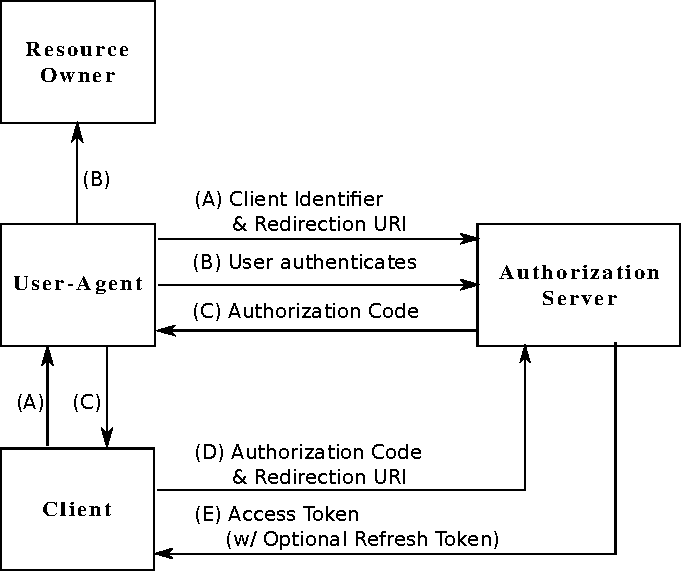
\includegraphics[width=\textwidth]{Oauth2.pdf}
  \caption{OAuth 2.0 protocol flow}
  \label{fig:oauth2flow}
\end{figure*}

\begin{enumerate}
\item resource owner -- An entity capable of granting access to a protected resource. When the resource owner is a person, it is referred to as an end-user (i.e. you).

\item resource server -- The server hosting the protected resources, capable of accepting and responding to protected resource requests using access tokens.

\item client -- An application which accesses a resource owner's protected resources after the resource owner has explicitly granted it permission -- this last part can also be rephrased into "after the resource owner has authorized the client to his/her protected resources".

\item authorization server -- The server issuing access tokens to the client after successfully authenticating the resource owner and obtaining authorization. The authorization server may be the same server as the resource server or a separate entity.
\end{enumerate}

The OAuth protocol flow in Fig.~\ref{fig:oauth2flow} can be explained as follows:

\paragraph*{(A)} The client initiates the flow by directing the resource owner's user-agent to the authorization endpoint. The client includes         its client identifier, requested scope, local state, and a redirection URI to which the authorization server will send the user-agent back once access is granted (or denied).

\paragraph*{(B)} The authorization server authenticates the resource owner (via the user-agent) and establishes whether the resource owner grants or denies the client's access request.

\paragraph*{(C)} Assuming the resource owner grants access, the authorization server redirects the user-agent back to the client using the redirection URI provided earlier (in the request or during client registration). The redirection URI includes an authorization code and any local state provided by the client earlier.

\paragraph*{(D)} The client requests an access token from the authorization server's token endpoint by including the authorization code received in the previous step. When making the request, the client authenticates with the authorization server. The client includes the redirection URI used to obtain the authorization code for verification.

\paragraph*{(E)} The authorization server authenticates the client, validates the authorization code, and ensures the redirection URI received matches the URI used to redirect the client in step (C). If valid, the authorization server responds back with an access token and optionally, a refresh token. A single access token may grant varying degrees of access to multiple APIs. The set of resources and operations permitted by an access token is controlled during the access token request via a variable parameter called \textit{scope}. Several scopes may be included in a request.\\

To summarize what we have seen so far, OAuth is not exactly an access delegation protocol, but rather a protocol which authorizes a resource consumer to securely access data from a resource server. Once the access token has been created, both applications communicate directly between themselves, without any need for delegation.

We can only assume that in a non-Linked Data environment, one can take advantage of OAuth in order to create the trust relationship between a user (agent) and the secretary (cf. Listing~\ref{list:sec_relation}), while access delegation would take place at a later time.

%As opposed to WebID Access Delegation where the resource owner specifies the secretary relation using Linked Data (cf. Listing~\ref{list:sec_relation})\todo{A: Linked Data reference?}, OAuth requires a pre-existing relationship between resource consumer and resource server, in the form of a shared secret. The OAuth relationship is created by manually registering \textit{each} resource consumer with the resource server. Furthermore, explicit user consent is required each time a new resource consumer requires access to the user's resource server.

%A fix for cases where there is little trust in a secretary, or when bootstrapping a user's server. The resource provider can store the request from consumer, and send a pingback to the consumer service, to notify him/her of a pending authorization request from consumer. Then the user will have to authenticate personally (through the browser, in order to verify the private key) to the provider, check a list of pending requests for his/her WebID, and decide if the request in question is valid or not. In other words, the user must give his/her consent if the secretary's identity is unknown to the provider.

\subsection{Cross Origin Resource Sharing (CORS)}
\todo{Henry Story: Compare to CORS in the context of Consuming Linked Data}



\bibliographystyle{plain}
\bibliography{webid}

\end{document}
